\subsection{Diagrama de Gantt}

\begin{figure}[!htp]
	\centering
	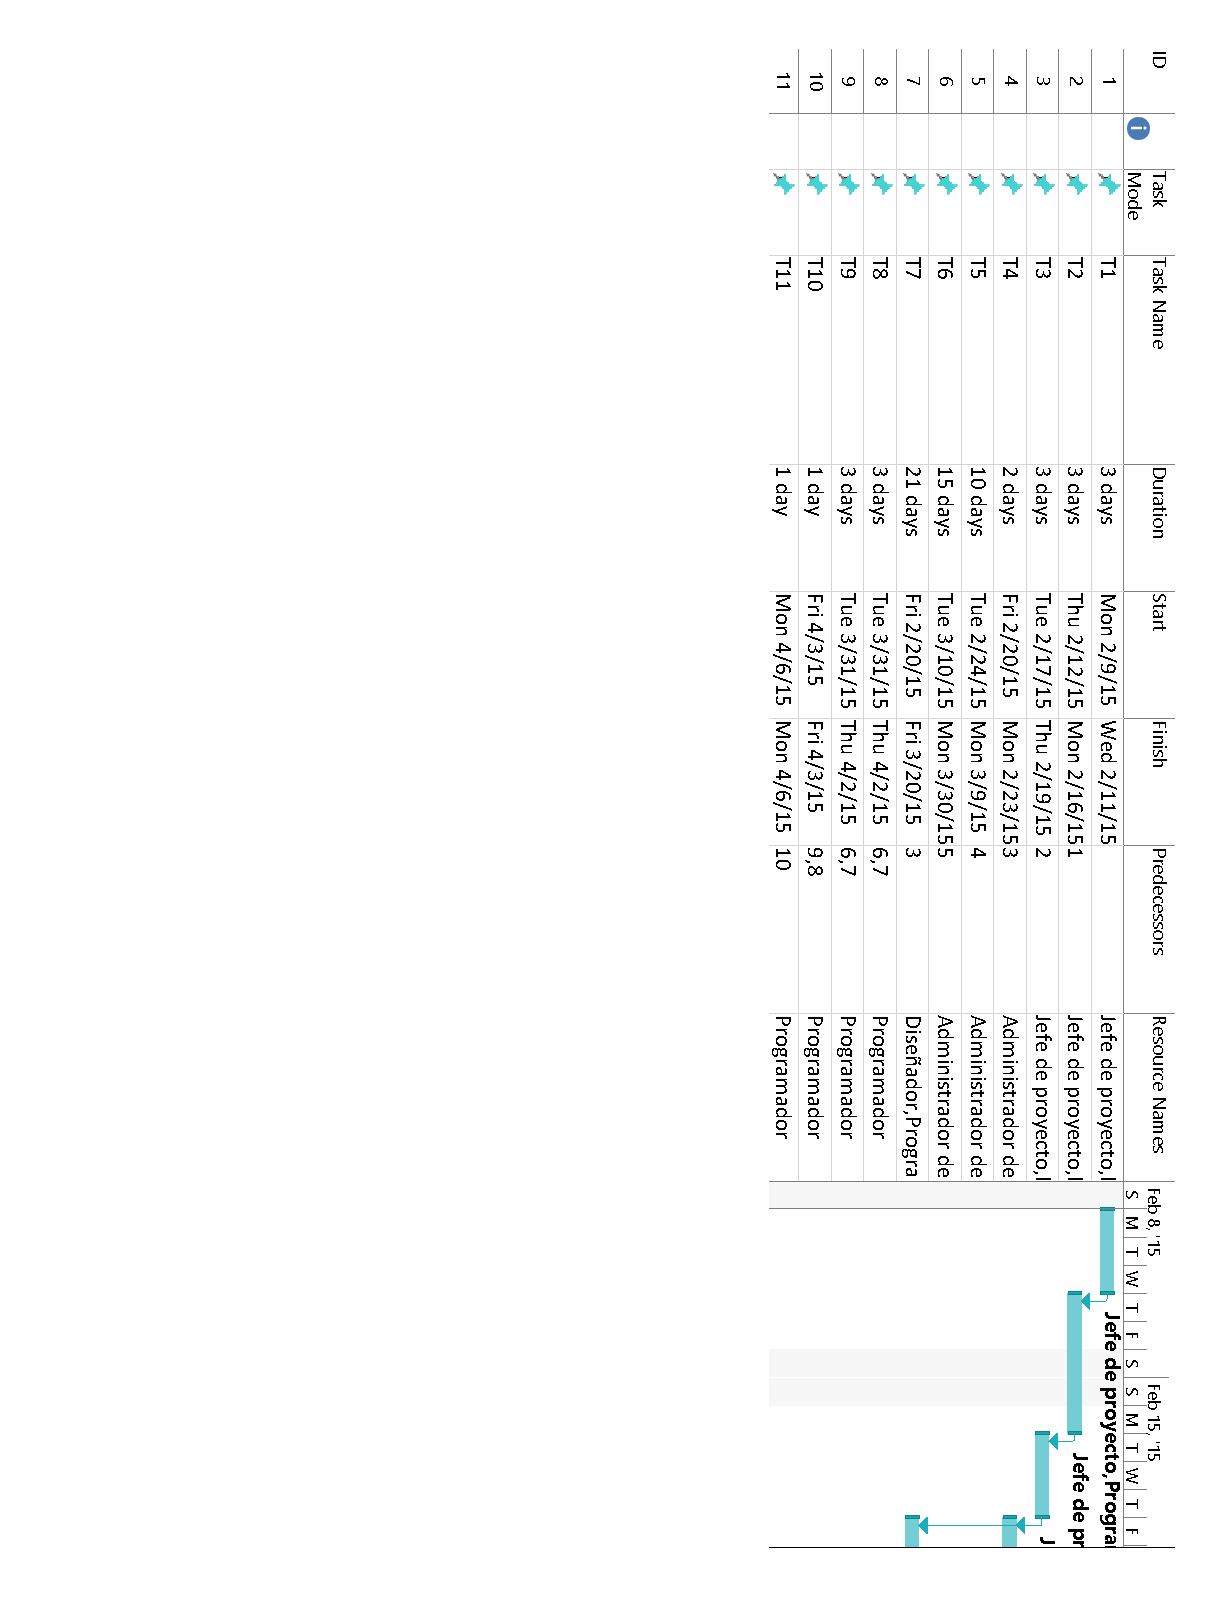
\includegraphics[page=1, scale=.7]{fig/gantt_diagram}
	\caption{Diagrama de Gantt 1}
\end{figure}

\begin{figure}[!htp]
	\centering
	\includegraphics[page=2, scale=.7]{fig/gantt_diagram}
	\caption{Diagrama de Gantt 2}
\end{figure}

\begin{figure}[!htp]
	\centering
	\includegraphics[page=3, scale=.7]{fig/gantt_diagram}
	\caption{Diagrama de Gantt 3}
\end{figure}

\begin{figure}[!htp]
	\centering
	\includegraphics[page=4, scale=.7]{fig/gantt_diagram}
	\caption{Leyenda del diagrama de Gantt}
\end{figure}